\chapter{Preliminaries}

This chapter reviews the theoretical and empirical literature surrounding the core concepts of this research, namely AlphaZero, and its core components, the Monte-Carlo Tree Search, a deep neural network and reinforcement learning.

\section{Mathematical Concepts}

A set is a well-defined collection of objects (\cite{diestel2024graph}).

A function $f: X \to Y$ is a subset of $X \times Y$ such that for each $x \in X$, there is a unique $y \in Y$ such that $(x, y) $ is in the subset (\cite{thielman1953definition}).

The derivative of a function denoted by $f'(x)$ is defined by Equation \ref{eq:derivative} (\cite{kalanov2019definition}).

\begin{equation}
    f'(x) = \frac{df}{dx} = \lim_{h \to 0} \frac{f(x+h) - f(x)}{h}
    \label{eq:derivative}
\end{equation}

The partial derivative of a multivariable function $f(x_1, x_2, \ldots, x_n)$ with respect to $x_i$ for $1 \le i \le n$ denoted by $\dfrac{\partial f}{\partial x_i}$ is defined by Equation \ref{eq:partial-derivative} (\cite{widder2012advanced}).

\begin{equation}
    \frac{df}{\partial x_i} = \lim_{h \to 0} \frac{f(x_1, x_2, \ldots, x_i + h, \ldots, x_n) - f(x_1, x_2, \ldots, x_i, \ldots, x_n)}{h}
    \label{eq:partial-derivative}
\end{equation}

The gradient $\nabla$ of a multivariable function $f(x_1, x_2, \ldots, x_n)$ is defined by Equation \ref{eq:gradient} (\cite{calder2020calculus}). The gradient descent of a function $-\nabla f$ at point $p$ points to the direction for which $(p, f(p))$ has the highest descent.

\begin{equation}
    \nabla f = \left[\dfrac{\partial f}{\partial x_{1}}, \dfrac{\partial f}{\partial x_{2}}, \dfrac{\partial f}{\partial x_{3}}, \ldots, \dfrac{\partial f}{\partial x_{n}} \right]^T
    \label{eq:gradient}
\end{equation}

A graph $G$ is a pair of two sets $(V, E)$ where $V$ is a set whose elements are called vertices, and $E$ is the set of unordered pairs $\{v_i, v_j\}$ for any connected vertices $v_i, v_j \in V$, whose elements are called edges (\cite{diestel2024graph}).

\begin{figure}[htb]
    \centering
    \begin{subfigure}{0.4\textwidth}
        \centering
        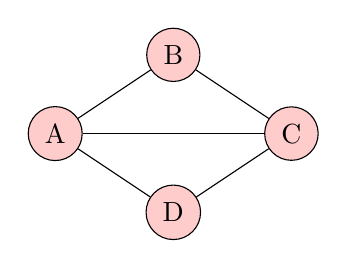
\begin{tikzpicture}
            \node[circle, draw, fill=red!20] (A) at (0, 1) {A};
            \node[circle, draw, fill=red!20] (B) at (1.5, 2) {B};
            \node[circle, draw, fill=red!20] (C) at (3, 1) {C};
            \node[circle, draw, fill=red!20] (D) at (1.5, 0) {D};
        
            \draw (A) -- (B);
            \draw (B) -- (C);
            \draw (C) -- (D);
            \draw (D) -- (A);
            \draw (A) -- (C);
        \end{tikzpicture}
        \caption{Undirected Graph}
        \label{fig:undirected-graph}
    \end{subfigure}
    \qquad
    \begin{subfigure}{0.4\textwidth}
        \centering
        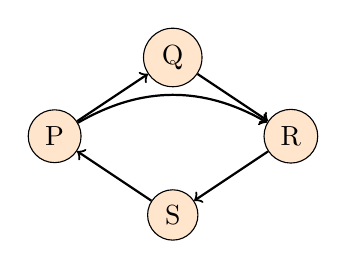
\begin{tikzpicture}
            \node[circle, draw, fill=orange!20] (P) at (5, 1) {P};
            \node[circle, draw, fill=orange!20] (Q) at (6.5, 2) {Q};
            \node[circle, draw, fill=orange!20] (R) at (8, 1) {R};
            \node[circle, draw, fill=orange!20] (S) at (6.5, 0) {S};
        
            \draw[->, thick] (P) -- (Q);
            \draw[->, thick] (Q) -- (R);
            \draw[->, thick] (R) -- (S);
            \draw[->, thick] (S) -- (P);
            \draw[->, thick] (P) to[bend left] (R);
        \end{tikzpicture}
        \caption{Directed Graph}
        \label{fig:directed-graph}
    \end{subfigure}
    \caption{Examples of Graph}
\end{figure}

A graph is said to be undirected if the edges are unordered as shown in Figure \ref{fig:undirected-graph}. That is, for all $\{v_i, v_j\} \in E, \{v_j, v_i\}\neq \{v_j, v_i\}$. Otherwise, it is called a directed graph as shown in Figure \ref{fig:directed-graph} (\cite{diestel2024graph}).

A graph is connected if for any two vertices $v_i, v_j \in V$, there exists at least one path connecting $v_i$ and $v_i$ (\cite{diestel2024graph}).

A walk is a sequence of vertices $v_1, v_2, \ldots, v_k \in V$ such that $\{v_i, v_{i+1}\} \in E$ for $1 \le i \le k$. A path is a walk with distinct vertices and edges as shown in Figure \ref{fig:path}. A cycle is a walk that starts and ends on the same vertex, it also has distinct vertices and edges with the exception of the last vertex as shown if Figure \ref{fig:cycle}. If a graph does not have a cycle, then it is called acyclic (\cite{diestel2024graph}).

\begin{figure}[htb]
    \centering
    \begin{subfigure}{0.4\textwidth}
        \centering
        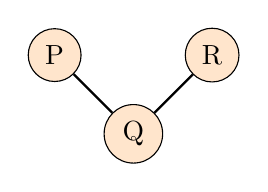
\begin{tikzpicture}
            \node[circle, draw, fill=orange!20] (P1) at (5, -4) {P};
            \node[circle, draw, fill=orange!20] (P2) at (6, -5) {Q};
            \node[circle, draw, fill=orange!20] (P3) at (7, -4) {R};
            \draw[thick] (P1) -- (P2) -- (P3);
        \end{tikzpicture}
        \caption{Path}
        \label{fig:path}
    \end{subfigure}
    \qquad
    \begin{subfigure}{0.4\textwidth}
        \centering
        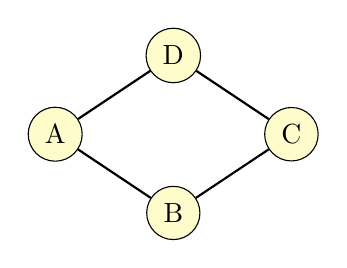
\begin{tikzpicture}
            \node[circle, draw, fill=yellow!20] (C1) at (0, -4) {A};
            \node[circle, draw, fill=yellow!20] (C2) at (1.5, -5) {B};
            \node[circle, draw, fill=yellow!20] (C3) at (3, -4) {C};
            \node[circle, draw, fill=yellow!20] (C4) at (1.5, -3) {D};
            \draw[thick] (C1) -- (C2) -- (C3) -- (C4) -- (C1);
        \end{tikzpicture}
        \caption{Cycle}
        \label{fig:cycle}
    \end{subfigure}
    \caption{Example of a Path and Cycle}
\end{figure}

A tree is an undirected graph that is connected and acyclic (\cite{diestel2024graph}). A rooted tree is a tree in which one vertex has been designated as the root. A leaf of a tree is a vertex that is connected to one vertex at most.

\begin{figure}[htb]
    \centering
    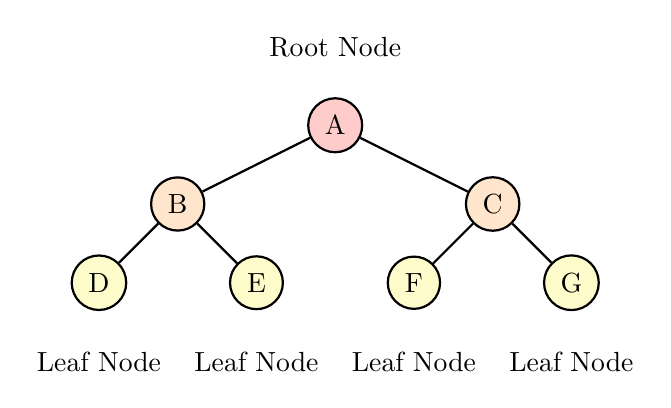
\begin{tikzpicture}
        \node[circle, draw, fill=red!20, thick] (A) at (0, 2) {A};
        \node[circle, draw, fill=orange!20, thick] (B) at (-2, 1) {B};
        \node[circle, draw, fill=orange!20, thick] (C) at (2, 1) {C};
        \node[circle, draw, fill=yellow!20, thick] (D) at (-3, 0) {D};
        \node[circle, draw, fill=yellow!20, thick] (E) at (-1, 0) {E};
        \node[circle, draw, fill=yellow!20, thick] (F) at (1, 0) {F};
        \node[circle, draw, fill=yellow!20, thick] (G) at (3, 0) {G};
        
        \node[above of=A] {\text{Root Node}};
        \node[below of=D] {\text{Leaf Node}};
        \node[below of=E] {\text{Leaf Node}};
        \node[below of=F] {\text{Leaf Node}};
        \node[below of=G] {\text{Leaf Node}};
        
        \draw[thick] (A) -- (B) -- (D);
        \draw[thick] (B) -- (E);
        \draw[thick] (A) -- (C) -- (F);
        \draw[thick] (C) -- (G);
    \end{tikzpicture}
    \caption{Example of a Tree}
\end{figure}

\section{Machine Learning Concepts}

A neural network is a function $f_\theta$ that maps the set of inputs $X$ to a set of outputs $Y$ with parameters $\theta$ (\cite{gurney2018introduction}).

An example of a neural network is an image classifier. An image classifier takes an input image $x \in X$, such as a handwritten digit, and maps it to a probability vector $f(x) \in Y$. This probability vector represents the likelihood of the image belonging to each possible class (\cite{kadam2020cnn}). 

\begin{figure}[htb]
    \centering
    \begin{equation*}
        f\left(\begin{gathered} 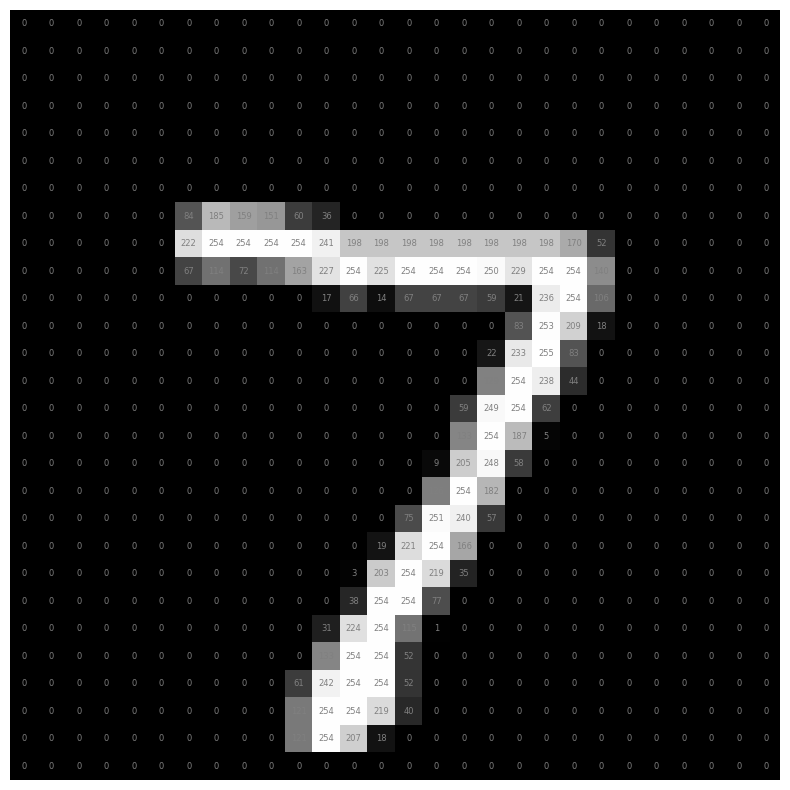
\includegraphics[width=0.28\linewidth]{images/neural_network_input_space.png} \end{gathered}\right) = \begin{bmatrix}
            \color{black!5} 0.0500 \\
            \color{black!5} 0.0500 \\
            \color{black!10} 0.1000 \\
            \color{black!20} 0.2000 \\
            \color{black!5} 0.0500 \\
            \color{black!1} 0.0100 \\
            \color{black!5} 0.0500 \\
            \color{black!47} 0.4700 \\
            \color{black!1} 0.0100 \\
            \color{black!1} 0.0100
        \end{bmatrix}
    \end{equation*}
    \caption{Example of a Neural Network Inference}
    \label{fig:nn-function}
\end{figure}

The image can be represented as a two-dimensional $28 \times 28$ matrix, where each element represents the luminosity of the pixel value. As shown in Figure \ref{fig:nn-function}, the function $f$ outputs a $1 \times 10$ probability vector where the zero-based index of the largest element represents what is the predicted value for the digit. In this case the highest value is at the $7^{th}$ position, then this means that the predicted value is the number $7$. 

% Here the neural network trains from a set $D$ composed of tuples with the first element being an image of a number represented as a $28\times 28$ matrix and the second one being the one-hot encoding representation of that number.

% One-hot encoding refers to the 

Neural networks are made up of one or more layers. Each layer accepts an input from previous layers and applies a differentiable function.

A linear layer applies the \verb|Linear| function defined by Equation \ref{eq:linear} to the input where $W$ is the weight matrix and $b$ is the bias vector. Both $W$ and $b$ are learnable parameters. The dimensions of the output of a linear layer depends on the dimensions of $W$ which can be configured. A linear layer is also called a dense layer.

\begin{equation}
    \verb|Linear|(x) = xW^T + b
    \label{eq:linear}
\end{equation}

A two-dimensional convolution layer applies the \verb|Conv2D| function defined by Equation \ref{eq:2dconvolution} where $x$ is the two-dimensional input represented as an $n \times m$ matrix, $b$ is the bias matrix, $(p_u, p_v)$ is the padding, and $W$ is the convolution matrix also known as the kernel with indexes from $-k_u$ to $k_u$ and $-k_v$ to $k_v$ for each dimension respectively. Both $W$ and $b$ are learnable parameters. The dimensions of the output of a two-dimensional convolution layer depends on the dimensions of $W$ which can be configured according to \cite{DBLP:journals/corr/OSheaN15}

\begin{equation}
    \verb|Conv2D|(x) = b + \sum_{u = p_u}^{n - p_u} \sum_{v = p_v}^{m - p_v} \sum_{\delta_u = -k_u}^{k_u} \sum_{\delta_v = -k_v}^{k_v} W(\delta_u, \delta_v) \cdot x(u + \delta_u, v + \delta_v)
    \label{eq:2dconvolution}
\end{equation}

A batch normalization layer applies the \verb|BatchNormalization| function defined by Equation \ref{eq:batch-normalization} to the input where $\gamma$ and $\beta$ are learnable parameters and $\epsilon$ is a small number typically equal to $1\times 10^{-5}$ (\cite{chollet2015keras}).

\begin{equation}
    \verb|BatchNormalization|(x) = \gamma \cdot \frac{x - \text{mean}{(x)}}{\sqrt{\text{variance}(x) + \epsilon}} + \beta
    \label{eq:batch-normalization}
\end{equation}

Activation layers applies a function to each element of the input. Non-linear activation layers introduces non-linearity to neural networks. Non-linear activation layers allows the neural network to model non-linear data (\cite{activation}).

A rectified linear unit (ReLU) layer is a non-linear activation layer that applies the \verb|ReLU| function defined by Equation \ref{eq:relu} to each of the element of its input (\cite{activation}). 

\begin{equation}
    \verb|ReLU|(x) =  \max\{0, x\}
    \label{eq:relu}
\end{equation}

A leaky ReLU layer is a generalization of the ReLU layer. A leaky ReLU is a non-linear activation layer that applies the \verb|LeakyReLU| function defined by Equation \ref{eq:leakyrelu} where $s$ is the slope of the values below $0$. When $s=0$, the leaky ReLU layer simplifies to the ReLU layer (\cite{activation}).

\begin{equation}
    \verb|LeakyReLU|(x) = \max{\{0, x\}} + s \cdot \min{\{0, x\}}
    \label{eq:leakyrelu}
\end{equation}

A flatten layer takes an input $x$ of any dimension and transforms it into a 1-dimensional array (\cite{chollet2015keras}).

% convolutional neural networks
% Similar to the paper by \cite{silver2017masteringchessshogiselfplay}, the model of \cite{Popic_Boskovic_Brest_2021} is a deep convolutional neural network (CNN). A CNN is a type of neural network that specializes on image classification due to their ability to recognize patterns in images. The rationale is that the model can learn to evaluate the positions of the pieces on the board and make appropriate moves accordingly because it is a CNN. 

% The main component of a CNN is a convolution layer. It

% As denoted in \cite{Popic_Boskovic_Brest_2021} the model contains convolution layers followed by normalization layers to stabilize the inputs and make the training faster and more stable. This layer is also called  called batch normalization as denoted by ``Normalization'' in Figure \ref{fig:popic-nn}.

\section{Training}

Training refers to the process of fitting the neural network to a set $D = \{ (x,\hat{y}) \mid x \in X, \hat{y} \in Y\}$ by minimizing a loss function $L(y, \hat{y})$ where $y = f(x)$ and $\hat{y}$ is the expected value of $f(x)$. The output of the neural network $y$ should converge to the expected value $\hat{y}$ within a certain loss $L$. 

A loss function is a function that calculates the divergence of the predicted value of the network $y$ by the true value $\hat{y}$ in the set $D$ (\cite{loss}). As opposed to layers, loss functions are not part of the neural network and are simply a means to evaluate the performance of the neural network.

Categorical cross-entropy is a loss function defined by Equation \ref{eq:cce}.

\begin{equation}
    \verb|CategoricalCrossEntropy| = -\sum_{i=1}^{n} \hat{y_i} \log y_i
    \label{eq:cce}
\end{equation}

Mean squared error is a loss function defined by Equation \ref{eq:mse}.

\begin{equation}
    \verb|MeanSquaredError| = \frac{1}{n}\sum_{i=1}^{n} (y_i - \hat{y_i})^{2}
    \label{eq:mse}
\end{equation}

L2 regularization is a loss function that penalizes high-value parameters in a neural network defined by Equation \ref{eq:l2} where $\lambda$ is the regularization constant.

\begin{equation}
    \verb|L2| = \lambda \sum_{i=1}^n\theta_i^2
    \label{eq:l2}
\end{equation}

Minimizing a loss function involves computing the gradients of each parameter of each layer of the neural network. Internally, modern machine learning libraries such as TensorFlow and PyTorch uses the backpropagation algorithm to achieve this (\cite{pytorch}).

The backpropagation algorithm first builds a directed acyclic graph of computation which is built during the forward pass and uses this structure to compute the gradient of each parameter. For instance, suppose $L = x + \sin(xy)$, to adjust the parameters $x$ and $y$ we need to compute $\dfrac{\partial L}{\partial x}$ and $\dfrac{\partial L}{\partial y}$.

\begin{figure}[htb]
    \centering
    \begin{subfigure}{0.4\textwidth}
        \centering
        \begin{tikzpicture}
            \node[circle, draw, fill=red!20, thick] (x) at (1, 0) {$x$};
            \node[circle, draw, fill=red!20, thick] (y) at (5, 0) {$y$};
            \node[circle, draw, fill=orange!20, thick] (f1) at (3, -1) {$f_1$};
            \node[circle, draw, fill=orange!20, thick] (f2) at (3, -4) {$f_2$};
            \node[circle, draw, fill=yellow!20, thick] (L) at (3, -7) {$L$};
            
            \draw[thick, -stealth] (x) -- (f1);
            \draw[thick, -stealth] (y) -- (f1);
            \draw[thick, -stealth] (x) -- (L);
            \draw[thick, -stealth] (f1) -- (f2);
            \draw[thick, -stealth] (f2) -- (L);
            
            \node[right = 1.5mm of f1] (f1_label) {$f_1 = xy$};
            \node[right = 1.5mm of f2] (f2_label) {$f_2 = \sin f_1$};
            \node[right = 1.5mm of L] (f2_label) {$L= x + f_2$};
        \end{tikzpicture}
        \caption{Forward Pass}
        \label{fig:forward}
    \end{subfigure}
    \qquad
    \begin{subfigure}{0.4\textwidth}
        \centering
        \begin{tikzpicture}
            \node[circle, draw, fill=red!20, thick] (x) at (1, 0) {$x$};
            \node[circle, draw, fill=red!20, thick] (y) at (5, 0) {$y$};
            \node[circle, draw, fill=orange!20, thick] (f1) at (3, -1) {$f_1$};
            \node[circle, draw, fill=orange!20, thick] (f2) at (3, -4) {$f_2$};
            \node[circle, draw, fill=yellow!20, thick] (L) at (3, -7) {$L$};
            
            \draw[thick, -stealth] (f1) -- node[above] {$\dfrac{\partial f_1}{\partial x} = y$} (x);
            \draw[thick, -stealth] (f1) -- node[above] {$\dfrac{\partial f_1}{\partial y} = x$} (y);
            \draw[thick, -stealth] (f2) -- node[right] {$\dfrac{\partial f_2}{\partial f_1} = \cos f_1$} (f1);
            \draw[thick, -stealth] (L) -- node[left] {$\dfrac{\partial L}{\partial x} = 1$} (x);
            \draw[thick, -stealth] (L) -- node[right] {$\dfrac{\partial L}{\partial f_2} = 1$} (f2);
        \end{tikzpicture}
        \caption{Backward Pass}
        \label{fig:backward}
    \end{subfigure}
    \caption{Anatomy of a Backpropagation}
    \label{fig:gradients}
\end{figure}

Backpropagation takes advantage of the fact that the partial derivative of a function with respect to a variable $x$, can be written in terms of the intermediate derivatives of each function, as shown in \ref{fig:backward}. In that example, 

\begin{equation}
    \frac{\partial L}{\partial x} = \frac{\partial L}{\partial x} + \frac{\partial L}{\partial f_2} \frac{\partial f_2}{\partial f_1} \frac{\partial f_1}{\partial x} = 1 + y\cos{xy}
\end{equation}

\begin{equation}
    \frac{\partial L}{\partial y} =\frac{\partial L}{\partial f_2} \frac{\partial f_2}{\partial f_1} \frac{\partial f_1}{\partial y} = x\cos{xy}
\end{equation}

An optimizer is an algorithm that adjusts the weights of each parameter to minimize the loss.

The Stochastic Gradient Descent (\verb|SGD|) with Momentum shown in Algorithm \ref{alg:sgdm} is an optimizer that replaces the actual gradient of the loss calculated from the entire set of data by an estimate calculated from a randomly selected subset of the data. The momentum keeps track of the update to the parameters at each iteration and determines the next update as a linear combination of the gradient and the previous update.

\begin{algorithm}[htb]
\caption{Stochastic Gradient Descent with Momentum}
\label{alg:sgdm}
\begin{algorithmic}
    \Require The learning rate $\eta$, loss function $\mathcal{L}$, momentum $\rho$, and learnable parameters $\theta$ of each layers of the neural network.
    \State $\delta \gets \nabla \mathcal{L}$
    \Function{SGD}{$\eta$, $\mathcal{L}$, $\rho$, $\theta$}
        \State $\delta  \gets \rho \delta - \eta\nabla\mathcal{L}$ 
        \State $\theta \gets \theta - \delta $
    \EndFunction{}
\end{algorithmic}
\end{algorithm}

% \begin{algorithm}[htb]
% \caption{Training Loop}
% \begin{algorithmic}
%     \State $e \gets 0 $
%     \While{$e \le \text{EPOCHS}$}
%         \State $(x, \hat{y}) \gets \text{Random}(D)$ 
%         \State $y \gets f_{\theta}(x)$
%         \State $L \gets \mathcal{L}(y, \hat{y})$
%         \State \Call{Backpropagate}{$f_{\theta}$, $L$}
%         \State \Call{Optimizer}{$f_{\theta}$}
%         \State $e \gets e + 1$
%     \EndWhile
% \end{algorithmic}
% \end{algorithm}

\section{Game Tree}

A sequential game is a game in which each player takes turns, that is, one player chooses their own action before the others choose theirs. Perfect information means that each player in the game knows the full state of the game and the history leading up to that state. An example of a sequential game is Chess and Checkers.

Sequential games can be represented using game trees that capture various game states as vertices of the tree and the actions applied on the current game state as edges. The root node of the tree corresponds to the initial game state, and each edge represents a decision made by a player, leading to a new game state. All the leaf nodes represents a terminal game state wherein the game may be a win, a lose, or a draw for the players.

\begin{figure}[htb]
    \centering
    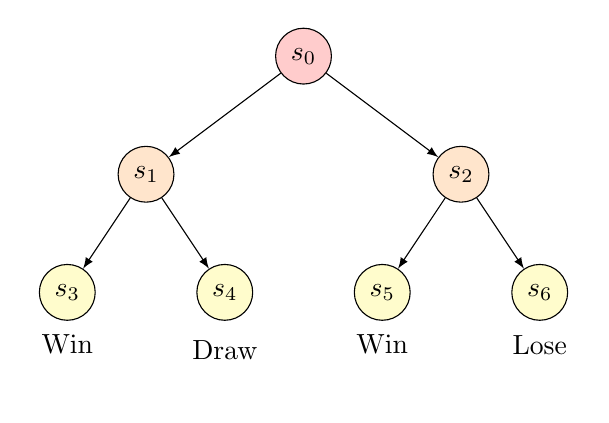
\begin{tikzpicture}[
      level 1/.style={sibling distance=40mm},
      level 2/.style={sibling distance=20mm},
      edge from parent/.style={draw,-latex},
      every node/.style={circle,draw,minimum size=7mm},
      label/.style={below=4pt, draw=none, fill=none}
      ]
      \node[fill=red!20] {$s_0$}
        child {node[fill=orange!20] {$s_1$}
          child {node[fill=yellow!20] {$s_3$} node[label] {Win}}
          child {node[fill=yellow!20] {$s_4$} node[label] {Draw}}
        }
        child {node[fill=orange!20] {$s_2$}
          child {node[fill=yellow!20] {$s_5$} node[label] {Win}}
          child {node[fill=yellow!20] {$s_6$} node[label] {Lose}}
        };
    \end{tikzpicture}
    \caption{Game Tree}
    \label{fig:game-tree}
\end{figure}

For simple games such as tic-tac-toe, all game states can be exhaustively analyzed by a computer and make it so that it produces the theoretically optimal winning move given a state. However, this is infeasible and computationally expensive for games such as Go and Chess. For instance, according to  \cite{jontromp}, the game of Go has been calculated to have approximately $2.1 \times 10^{170}$ possible moves, which is larger than the number of atoms in the universe. That means, it is  impossible to be approached this way. % cite

One approach to mitigate this is to approximate the optimal move by walking through only a finite nodes of the tree. Such an approach is employed by the AlphaZero framework and was used to beat professionals on games such as chess, go, and shogi.

\section{The AlphaZero Framework}

The AlphaZero framework is a general reinforcement learning algorithm by \cite{silver2017masteringchessshogiselfplay} that has shown success in conquering sequential games such as chess, go, and shogi. This framework can be applied to any sequential games with perfect information. This framework has three major components: the Monte-Carlo Tree Search Algorithm, a deep neural network, and reinforcement learning through self-play.

According to \cite{silver2017masteringchessshogiselfplay}, AlphaZero uses a general-purpose Monte-Carlo tree search (MCTS) algorithm. Each search consists of a series of simulated games of self-play that traverse a game tree from root $s_{root}$ to leaf. Each simulation proceeds by selecting in each state $s$ a move $a$ with low visit count $N(s, a)$, high move probability $P(s,a)$ and high value $Q(s, a)$ according to the current neural network $f_\theta$. The search returns a vector $\pi$ representing a probability distribution over moves, either proportionally or greedily with respect to the visit counts at the root state.

Each state-action pair $(s,a)$ stores a set of statistics, $\{N(s, a), W(s, a), Q(s, a), P(s, a)\}$, where $N(s, a)$ is the visit count, $W(s, a)$ is the total action-value, $Q(s, a)$ is the mean action-value, and $P(s, a)$ is the prior probability of selecting $a$ in $s$, as shown in Figure \ref{fig:game-tree-with-stats}.

\begin{figure}[htb]
    \centering
    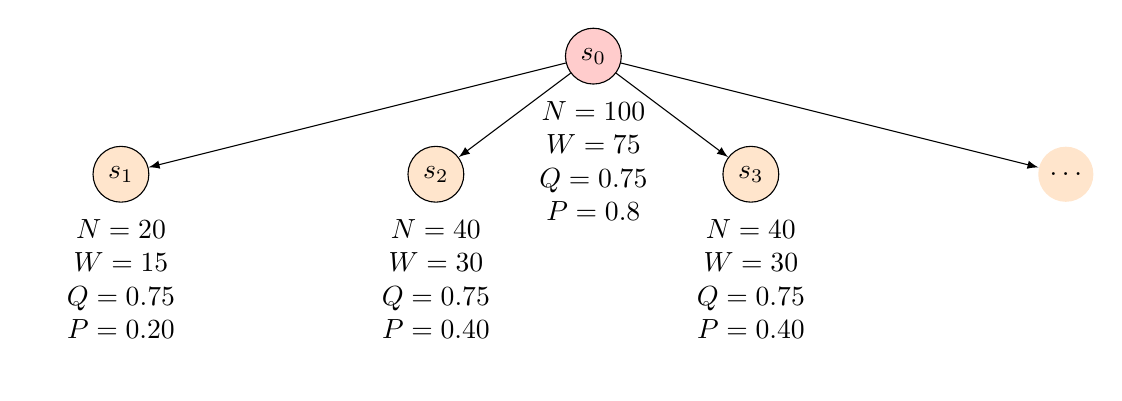
\begin{tikzpicture}[
      level 1/.style={sibling distance=40mm},
      level 2/.style={sibling distance=20mm},
      edge from parent/.style={draw,-latex},
      every node/.style={circle,draw,minimum size=7mm},
      label/.style={below=4pt, draw=none, fill=none, align=center}
      ]
      \node[label] {$N = 100$\\$W = 75$\\$Q = 0.75$\\$P = 0.8$} node[fill=red!20] {$s_0$}
        child {node[fill=orange!20] {$s_1$} node[label] {$N = 20$\\$W = 15$\\$Q = 0.75$\\$P = 0.20$}}
        child {node[fill=orange!20] {$s_2$} node[label] {$N = 40$\\$W = 30$\\$Q = 0.75$\\$P = 0.40$}}
        child {node[fill=orange!20] {$s_3$} node[label] {$N = 40$\\$W = 30$\\$Q = 0.75$\\$P = 0.40$}}
        child {node[fill=orange!20, draw=none] {$\dots$}};
    \end{tikzpicture}
    \caption{State-Action Pairs Storing a Set of Statistics}
    \label{fig:game-tree-with-stats}
\end{figure}

Each simulation begins at the root node of the search tree, $s_0$, and finishes when the simulation reaches a leaf node $s_L$ at time-step $L$, as shown in Figure \ref{fig:root-to-leaf}.

\begin{figure}[htb]
    \centering
    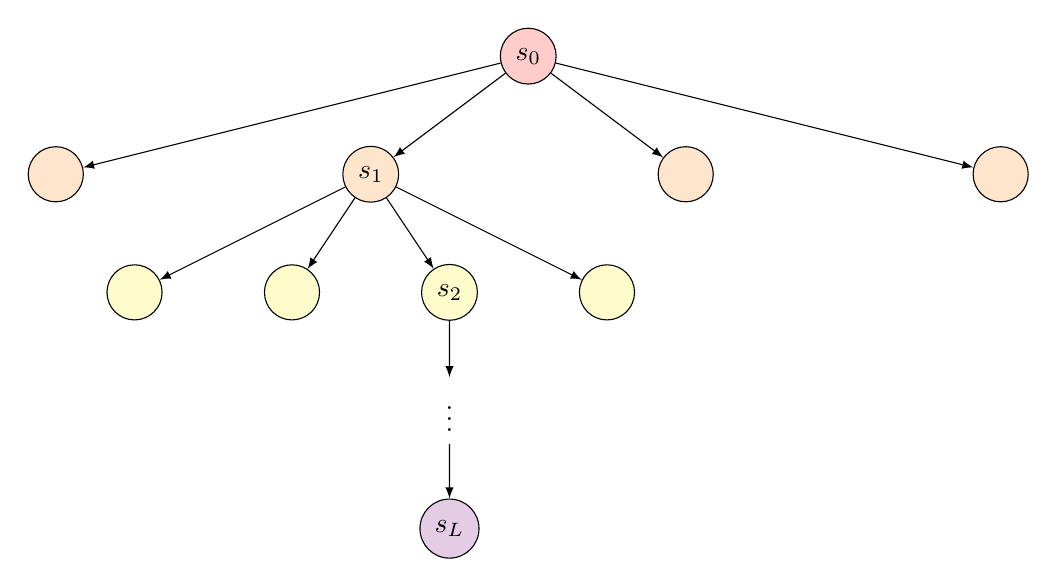
\begin{tikzpicture}[
      level 1/.style={sibling distance=40mm},
      level 2/.style={sibling distance=20mm},
      edge from parent/.style={draw,-latex},
      every node/.style={circle,draw,minimum size=7mm},
      label/.style={below=4pt, draw=none, fill=none, align=center}
      ]
      \node[fill=red!20] {$s_0$}
        child {node[fill=orange!20] {}}
        child {node[fill=orange!20] {$s_1$}
            child {node[fill=yellow!20] {}}
            child {node[fill=yellow!20] {}}
            child {node[fill=yellow!20] {$s_2$}
                child {node[draw=none] {$\vdots$}
                    child {node[fill=violet!20] {$s_L$}}}}
            child {node[fill=yellow!20] {}}}
        child {node[fill=orange!20] {}}
        child {node[fill=orange!20] {}};
    \end{tikzpicture}
    \caption{Simulation of MCTS on the Search Tree}
    \label{fig:root-to-leaf}
\end{figure}

At each of these time-steps, $t < L$, an action is selected $a_t = \operatorname{arg} \operatorname{max}_a \big(Q(s_t, a_t) + U(s_t, a_t)\big)$, using a variant of the Predictor + Upper-Confidence Bound Applied to Trees (PUCT) algorithm, $U(s, a) =  C(s) P(s, a) \sqrt{N(s)} / (1 + N(s, a))$, where $N(s)$ is the parent visit count and $C(s)$ is the exploration rate, which grows slowly with search time, $C(s) = \log\left((1 + N(s) + c_{base}) / c_{init}\right) + c_{init}$, but is essentially constant during the fast training games. The leaf node $s_L$ is added to a queue for neural network evaluation, $(\mathbf{p}, v) = f_\theta(s)$. The leaf node is expanded and each state-action pair $(s_L, a)$ is initialized to $\{N(s_L, a) = 0, W(s_L, a) = 0, Q(s_L, a) = 0, P(s_L, a) = p_a\}$. The visit counts and values are then updated in a backward pass through each step $t \leq L$, $N(s_t, a_t) = N(s_t, a_t) + 1$, $W(s_t, a_t) = W(s_t, a_t) + v$, $Q(s_t, a_t) = W(s_t,a_t) / N(s_t,a_t)$.

% During each search, a root node is The MCTS used in AlphaZero has four phases: selection, expansion, simulation, and backpropagation. The selection phase traverses the tree and make use of the Predictor + Upper-Confidence Bound Applied to Trees (PUCT) formula introduced by AlphaGo for the selection of nodes, balancing exploitation of nodes with higher estimated value with the exploration of least visited nodes. It continues down the tree until reaching a node that has not been fully expanded or explored. It does so by traversing through the nodes which has the largest PUCT score.

% $Q(s, a)$ is the average value of leaf states from the simulations that selected $a$ from $s$. 

% \begin{equation}\label{eq:q}
%     Q(s, a) = \frac{W(s, a)}{N(s, a)}
% \end{equation}
% \begin{equation}\label{eq:u}
%     U(s, a) = C(s) P(s, a) \sqrt{N(s)} \cdot \frac{1}{1 + N(s, a)}
% \end{equation}
% \begin{equation}\label{eq:cs}
%     C(s) = \log\left(\frac{1 + N(s) + c_{base}}{c_{init}}\right) + c_{init}
% \end{equation}

% The PUCT formula is defined by Equation \ref{eq:puct} where $C(s)$ is the exploration rate that grows slowly with the number of iterations $i$, $c_{base}$ and $c_{init}$ are constants chosen arbitrarily by AlphaZero, $v_i$ is the evaluated value of node $s$, $n_i$ is total number of visits of node $s$, and $N_i$ is the total number of visits of the parent node of $s$.

% \begin{equation}\label{eq:puct}
%     PUCT(s) = Q(s, a) + U(s, a)
% \end{equation}

% Once a node is selected, if it is not a terminal node, the algorithm generates one or more child nodes corresponding to possible moves from that state. This expands the tree by adding new game states for exploration.

% From the newly added node, the algorithm runs a random simulation of the game by selecting moves randomly until it reaches a terminal state. The outcome of the simulation (win, loss, draw, etc.) is recorded.

% The result of the simulation is then propagated back up the tree to update the statistics of the nodes along the path taken during selection. This step helps the algorithm adjust its understanding of which moves are more likely to result in favorable outcomes.

% Putting all these together we get the MCTS

% \begin{algorithm}[htb]
% \begin{algorithmic}[1]
%     \Function{MCTS}{$root, N_{max}$}
%         \State $N \gets 0$
%         \Repeat 
%             \State $leaf \gets \Call{Traverse}{root}$
%             \State $value \gets \Call{Simulate}{leaf}$
%             \State $\Call{Backpropagate}{leaf, value}$
%             \State $N \gets N + 1$
%         \Until{$N = N_{max}$}
%         \State \Return the child of $root$ with the highest number of visits
%     \EndFunction
% \end{algorithmic}
% \end{algorithm}

% \begin{algorithm}[htb]
% \begin{algorithmic}[1]
%     \Function{Traverse}{$node$}
%         \While{$node$ is a fully expanded node}
%             \State $node$ is assigned the child node of $node$ with the maximum PUCT score.
%         \EndWhile
%         \State \Return $\Call{UnvisitedChild}{node}$ or $node$
%     \EndFunction
% \end{algorithmic}
% \end{algorithm}

% \begin{algorithm}[htb]
% \begin{algorithmic}[1]
%     \Function{Simulate}{$node$}
%         \While{$node$ is a non-terminal node}
%             \State $node$ is assigned to a random children of $node$
%         \EndWhile
%         \State \Return $\Call{GetOutcome}{node}$
%     \EndFunction
% \end{algorithmic}
% \end{algorithm}

% \begin{algorithm}[htb]
% \begin{algorithmic}[l]
%     \Function{Backpropagate}{$node$, $value$}
%             \If{$node$ has no parent}
%                 \State \Return 
%             \EndIf

%             \State $\Call{UpdateParameters}{node, value}$
%             \State $\Call{Backpropagate}{\Call{GetParent}{node}, value}$
%     \EndFunction
% \end{algorithmic}
% \end{algorithm}

According to \cite{silver2017masteringchessshogiselfplay}, AlphaZero utilizes a deep neural network $(\mathbf{p}, v) = f_\theta(s)$ with parameters $\theta$. This neural network takes the board position $s$ as an input and outputs a vector of move probabilities $\mathbf{p}$ with components $p_a = Pr(a|s)$ for each action $a$, and a scalar value $v$ estimating the expected outcome $z$ from position $s$, $v \approx \mathbb{E}[z|s]$. AlphaZero learns these move probabilities and value estimates entirely from self-play; these are then used to guide its search.

According to \cite{silver2017masteringchessshogiselfplay}, the parameters $\theta$ of the deep neural network in AlphaZero are trained by self-play reinforcement learning, starting from randomly initialized parameters $\theta$. Games are played by selecting moves for both players by MCTS, $a_t \sim \mathbf{\pi}_t$. At the end of the game, the terminal position $s_T$ is scored according to the rules of the game to compute the game outcome $z$: $-1$ for a loss, $0$ for a draw, and $+1$ for a win. The neural network parameters $\theta$ are updated so as to minimize the error between the predicted outcome $v_t$ and the game outcome $z$, and to maximize the similarity of the policy vector $\mathbf{p}_t$ to the search probabilities $\pi_t$. Specifically, the parameters $\theta$ are adjusted by gradient descent on a loss function $l$ than sums over mean-squared error and cross-entropy losses respectively,

\begin{equation}\label{eq:loss}
    (\mathbf{p}, v) = f_\theta(s), \qquad l = (z - v)^2 - \pi^\top \log \mathbf{p} + c\lVert\theta\rVert^2
\end{equation}

where $c$ is a parameter controlling the level of $L_2$ weight regularisation. The updated parameters are used in subsequent games of self-play.

\section{Deep Learning and the Game of Checkers}

% paraphrase
Based on a study conducted by \cite{Popic_Boskovic_Brest_2021}, they were able to train a deep convolutional neural network based on the AlphaZero framework that was able to learn how to play the game of German checkers defined in their paper through self-play with each new version representing a better player. \cite{Popic_Boskovic_Brest_2021} focused on the rules of German checkers in which the game is played on an $8 \times 8$ board with interchanging black and white squares. There are 12 white and 12 black playing figures that are coin like shaped. Each player has their figures arranged on black squares in first 3 rows closest to them as shown in Figure \ref{fig:checkers-start}. 

\begin{figure}[htb]
    \centering
    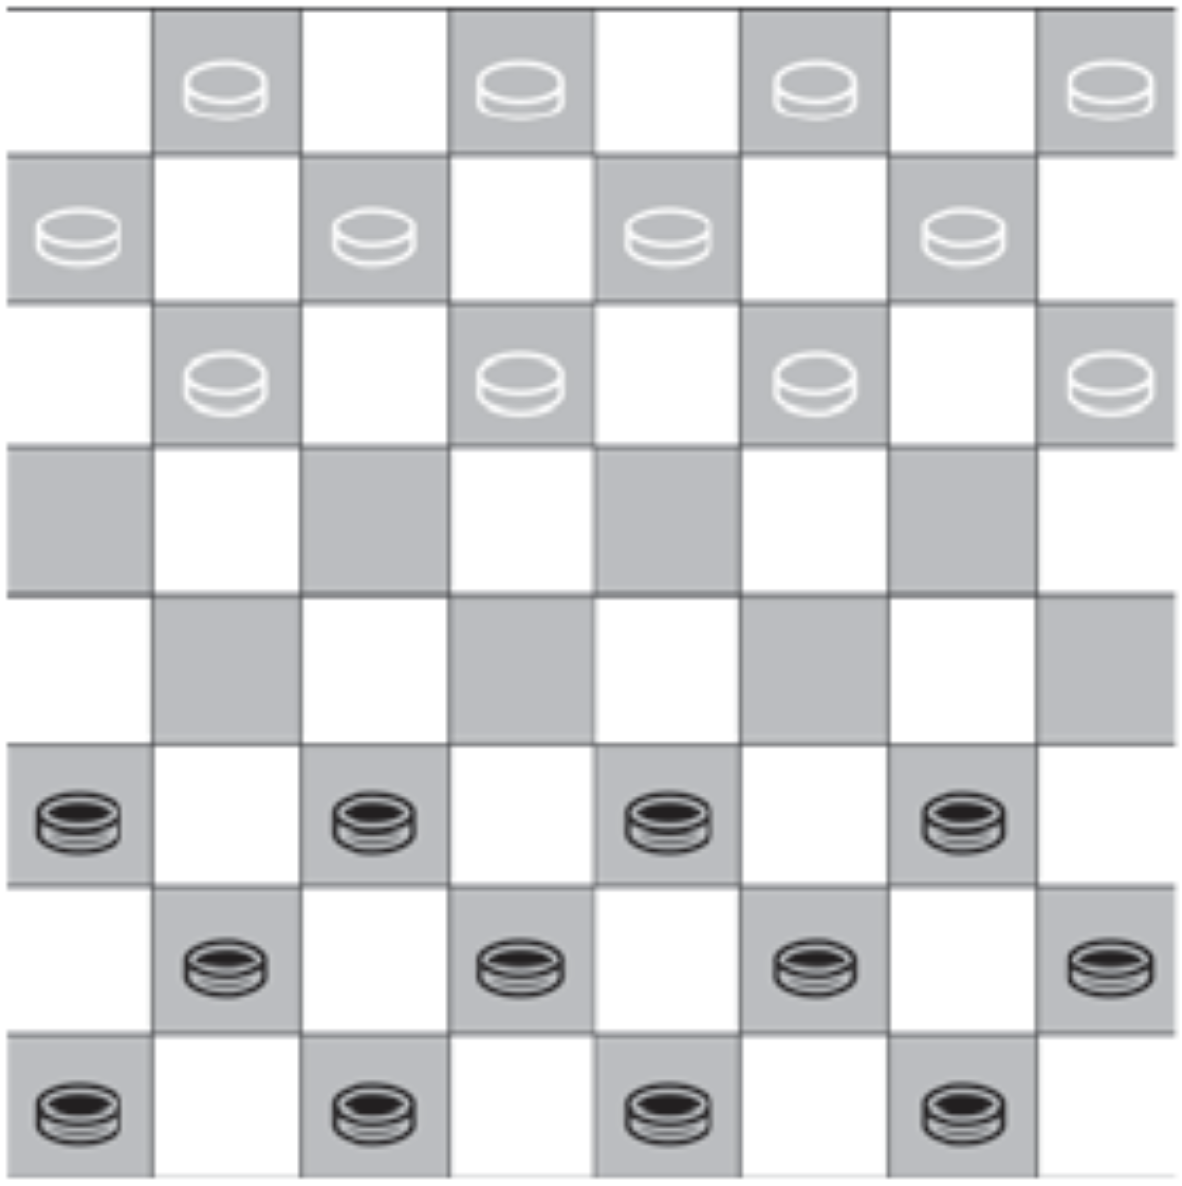
\includegraphics[width=0.3\textwidth]{images/checkers.png}
    \caption{Starting State of the Board in German Checkers used in \cite{Popic_Boskovic_Brest_2021}}
    \label{fig:checkers-start}
\end{figure}

A game of German checkers is always started by the player with black figures and is continued by the opponent. Regular game figures can only move diagonally on black squares towards the opponent’s side one square at a time. If there is an opponent’s figure in the path of the move and a square behind that figure is vacant, the player must capture the opponent’s figure by jumping over it and removing it from the playing board. If multiple such successive captures exist, the player must perform them all in one move.

If the player reaches the opponent’s side of the board, the player’s figure is knighted and gains the ability to move diagonally forward and backward for any number of squares at a time. A game is won if the opponent has no figures left on the board or is out of possible legal moves. The game ends in a draw if no pieces have been captured in the last 40 moves.

Two player agents with their own game tree and neural network were used in \cite{Popic_Boskovic_Brest_2021}. Each agent gets a list of possible legal moves it can make on its turn from the game environment. It also has a whole overview of the game state at any given time where it has full knowledge where the opponent has its figures and what type of figures they are.

\begin{table}[htb]
    \centering
    \begin{tabular}{lll}
        \hline
        Parameter & Value & Description \\ \hline
        \verb!EPISODES! & 50 & number of self-play games for data creation \\
        \verb!MCTS_SIMS! & 70 & number of MCTS iterations \\
        \verb!TURNS_UNTIL_TAU0! & 25 & number of moves after the game is played deterministically \\
        \verb!BATCH_SIZE! & 256 & batch size used for learning \\
        \verb!LEARNING_RATE! & 0.1 & learning rate \\
        \verb!MOMENTUM! & 0.9 & learning momentum \\
        \verb!EVAL_EPISODES! & 20 & number of games played in validation phase \\
        \verb!SCORING_THRESHOLD! & 1.3 & scoring factor in validation phase \\ \hline
    \end{tabular}
    \caption{Algorithm Parameters in \cite{Popic_Boskovic_Brest_2021}}
    \label{tab:algo-params}
\end{table}

During every turn, the agent uses the MCTS algorithm with parameters shown in Table \ref{tab:algo-params} to select the best move from the list of possible legal moves. Random move selection were used for the first \verb!TURNS_UNTIL_TAU0! game moves to further explore new and different game scenarios during the learning phase of the neural network.

Before the agent selects a move from the current game state $s$, the MCTS algorithm runs for \verb!MCTS_SIMS! iterations. Each node of the game tree represents a certain move $a$ and contains the number of node visits $N(s, a)$, its value $Q(s, a)$ and probability of selecting that move $P(s, a)$ received from the neural network. The current node value $Q(s, a)$ represents the mean value of its branch and is calculated from its leaf value $V(s^i_L)$ returned by the neural network, current node visit counter $N(s, a)$, and $l(s, a, i)$ which represents if the leaf $i$ was visited from the current node as shown in Equation \ref{eq:qsa}.

\begin{equation} \label{eq:qsa}
    Q(s, a) = \frac{1}{N(s,a)} \sum_i l(s, a, i) V(s^i_L) 
\end{equation}

The algorithm starts from the root node and continuously select moves $a$ that maximize the score $S(s, a) = Q(s, a) + u(s, a)$ where $u(s, a) \propto \frac{P(s,a)}{1+N(s,a)}$. $u(s, a)$ is used to improve the exploration of moves that have not been selected often and exploit moves that already have a sufficiently high prior probability $P(s, a)$ of being selected. During each node visit, the node's values are updated and the node's position are evaluated with the neural network if a leaf was reached. A move from the children of the root node which has the highest value $Q(s, a)$ is selected after \verb!MCTS_SIMS! iterations of tree traversal.

\begin{figure}[htb]
    \centering
    \begin{subfigure}{0.4\textwidth}
        \centering
        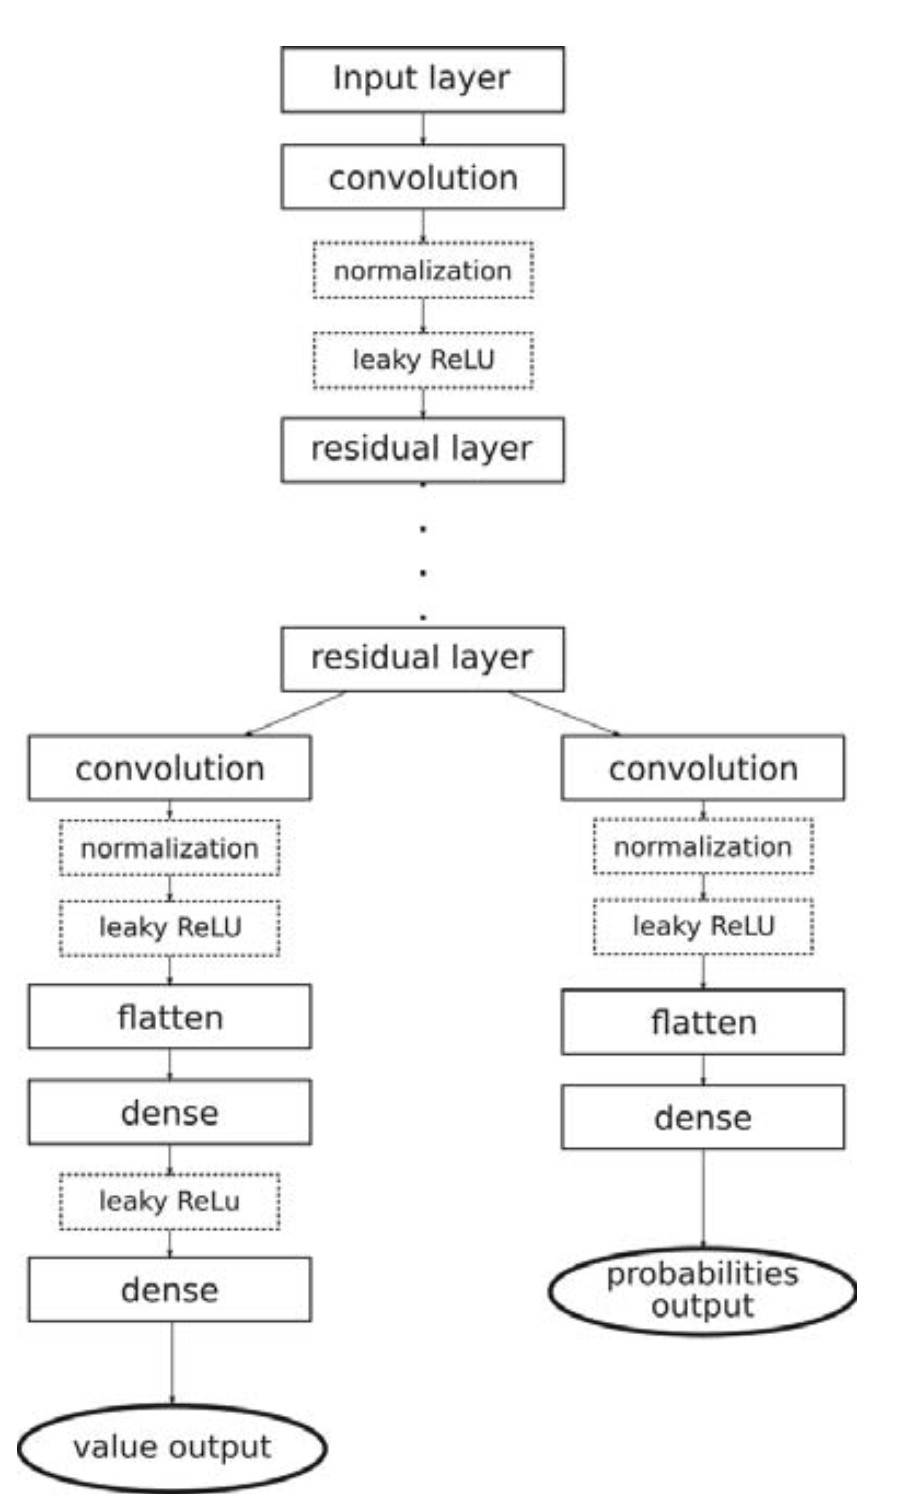
\includegraphics[scale=0.25]{images/checkers_nn.png}
        \caption{Deep Neural Network Architecture}
        \label{fig:dnn}
    \end{subfigure}
    \qquad
    \begin{subfigure}{0.4\textwidth}
        \centering
        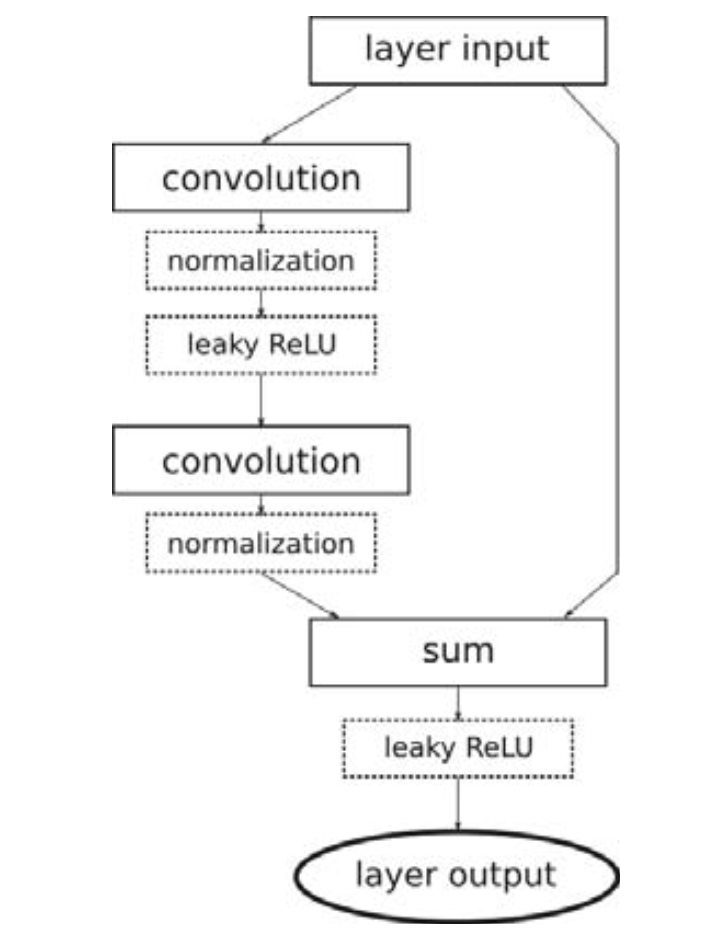
\includegraphics[scale=0.25]{images/residual_layer.png}
        \caption{Anatomy of a Residual Layer}
        \label{fig:residual}
    \end{subfigure}
    \caption{Overview of the Deep Neural Architecture used in \cite{Popic_Boskovic_Brest_2021}}
    \label{fig:popic-nn}
\end{figure}


The structure of the neural network used in \cite{Popic_Boskovic_Brest_2021} follows the architecture used in \cite{silver2017masteringchessshogiselfplay}. The input in the neural network is a matrix of size $2 \times 8 \times 8$ which describes the current game state, the first and second layer for the pieces of the first and second player, respectively. The numbers $-1$, $-2$, $1$, and $2$ are used to represent two different pieces for each player: normal and knighted pieces for white and black, respectively. After the input layer, there is a convolution layer with 75 kernels of size $4 \times 4$, followed by 5 residual layers. The overall structure is shown in Figure \ref{fig:dnn}.

Each residual layer consists of 2 convolutions with 75 kernels of size $4 \times 4$ followed by addition of this convolutions and layer input. Residual layer is represented in Figure \ref{fig:residual}. After every convolutional layer, the paper utilized batch normalization to speed up the learning and mitigate overfitting.

The neural network has 2 outputs. The first output is the result of a convolution layer, flattening layer and two dense layers which reduce the dimension to one value. This value represents value $V$ of the current board state. 
The second output is achieved by a convolution layer, that is again followed by flattening, and a dense layer which reduces the dimension to a vector of size 64. This represents the probability for each position. This output probability vector is of size 64 corresponding to the unraveled $8 \times 8$ board. This vector represents the probability distribution over possible new board states, not specific move pairs.

The neural network utilizes leaky ReLU activation function and stochastic gradient descend with momentum to adjust network weights and kernels.
x
The work in \cite{Popic_Boskovic_Brest_2021} consists of learning through self-play between two versions of the neural network. The general flow chart can be seen in Figure \ref{fig:self-play}. Data needed for learning is generated by playing a number of games provided by the \verb!EPISODES! parameter between an agent using the current neural network and an agent using the best neural network. Both neural networks are the same in the first iteration. During the data creation phase, every game is started by an agent that moves randomly, thus eliminating any advantage a starting player would have. After each game, the game states and normalized visit counts are saved from the MCTS algorithm.

\begin{figure}[htb]
    \centering
    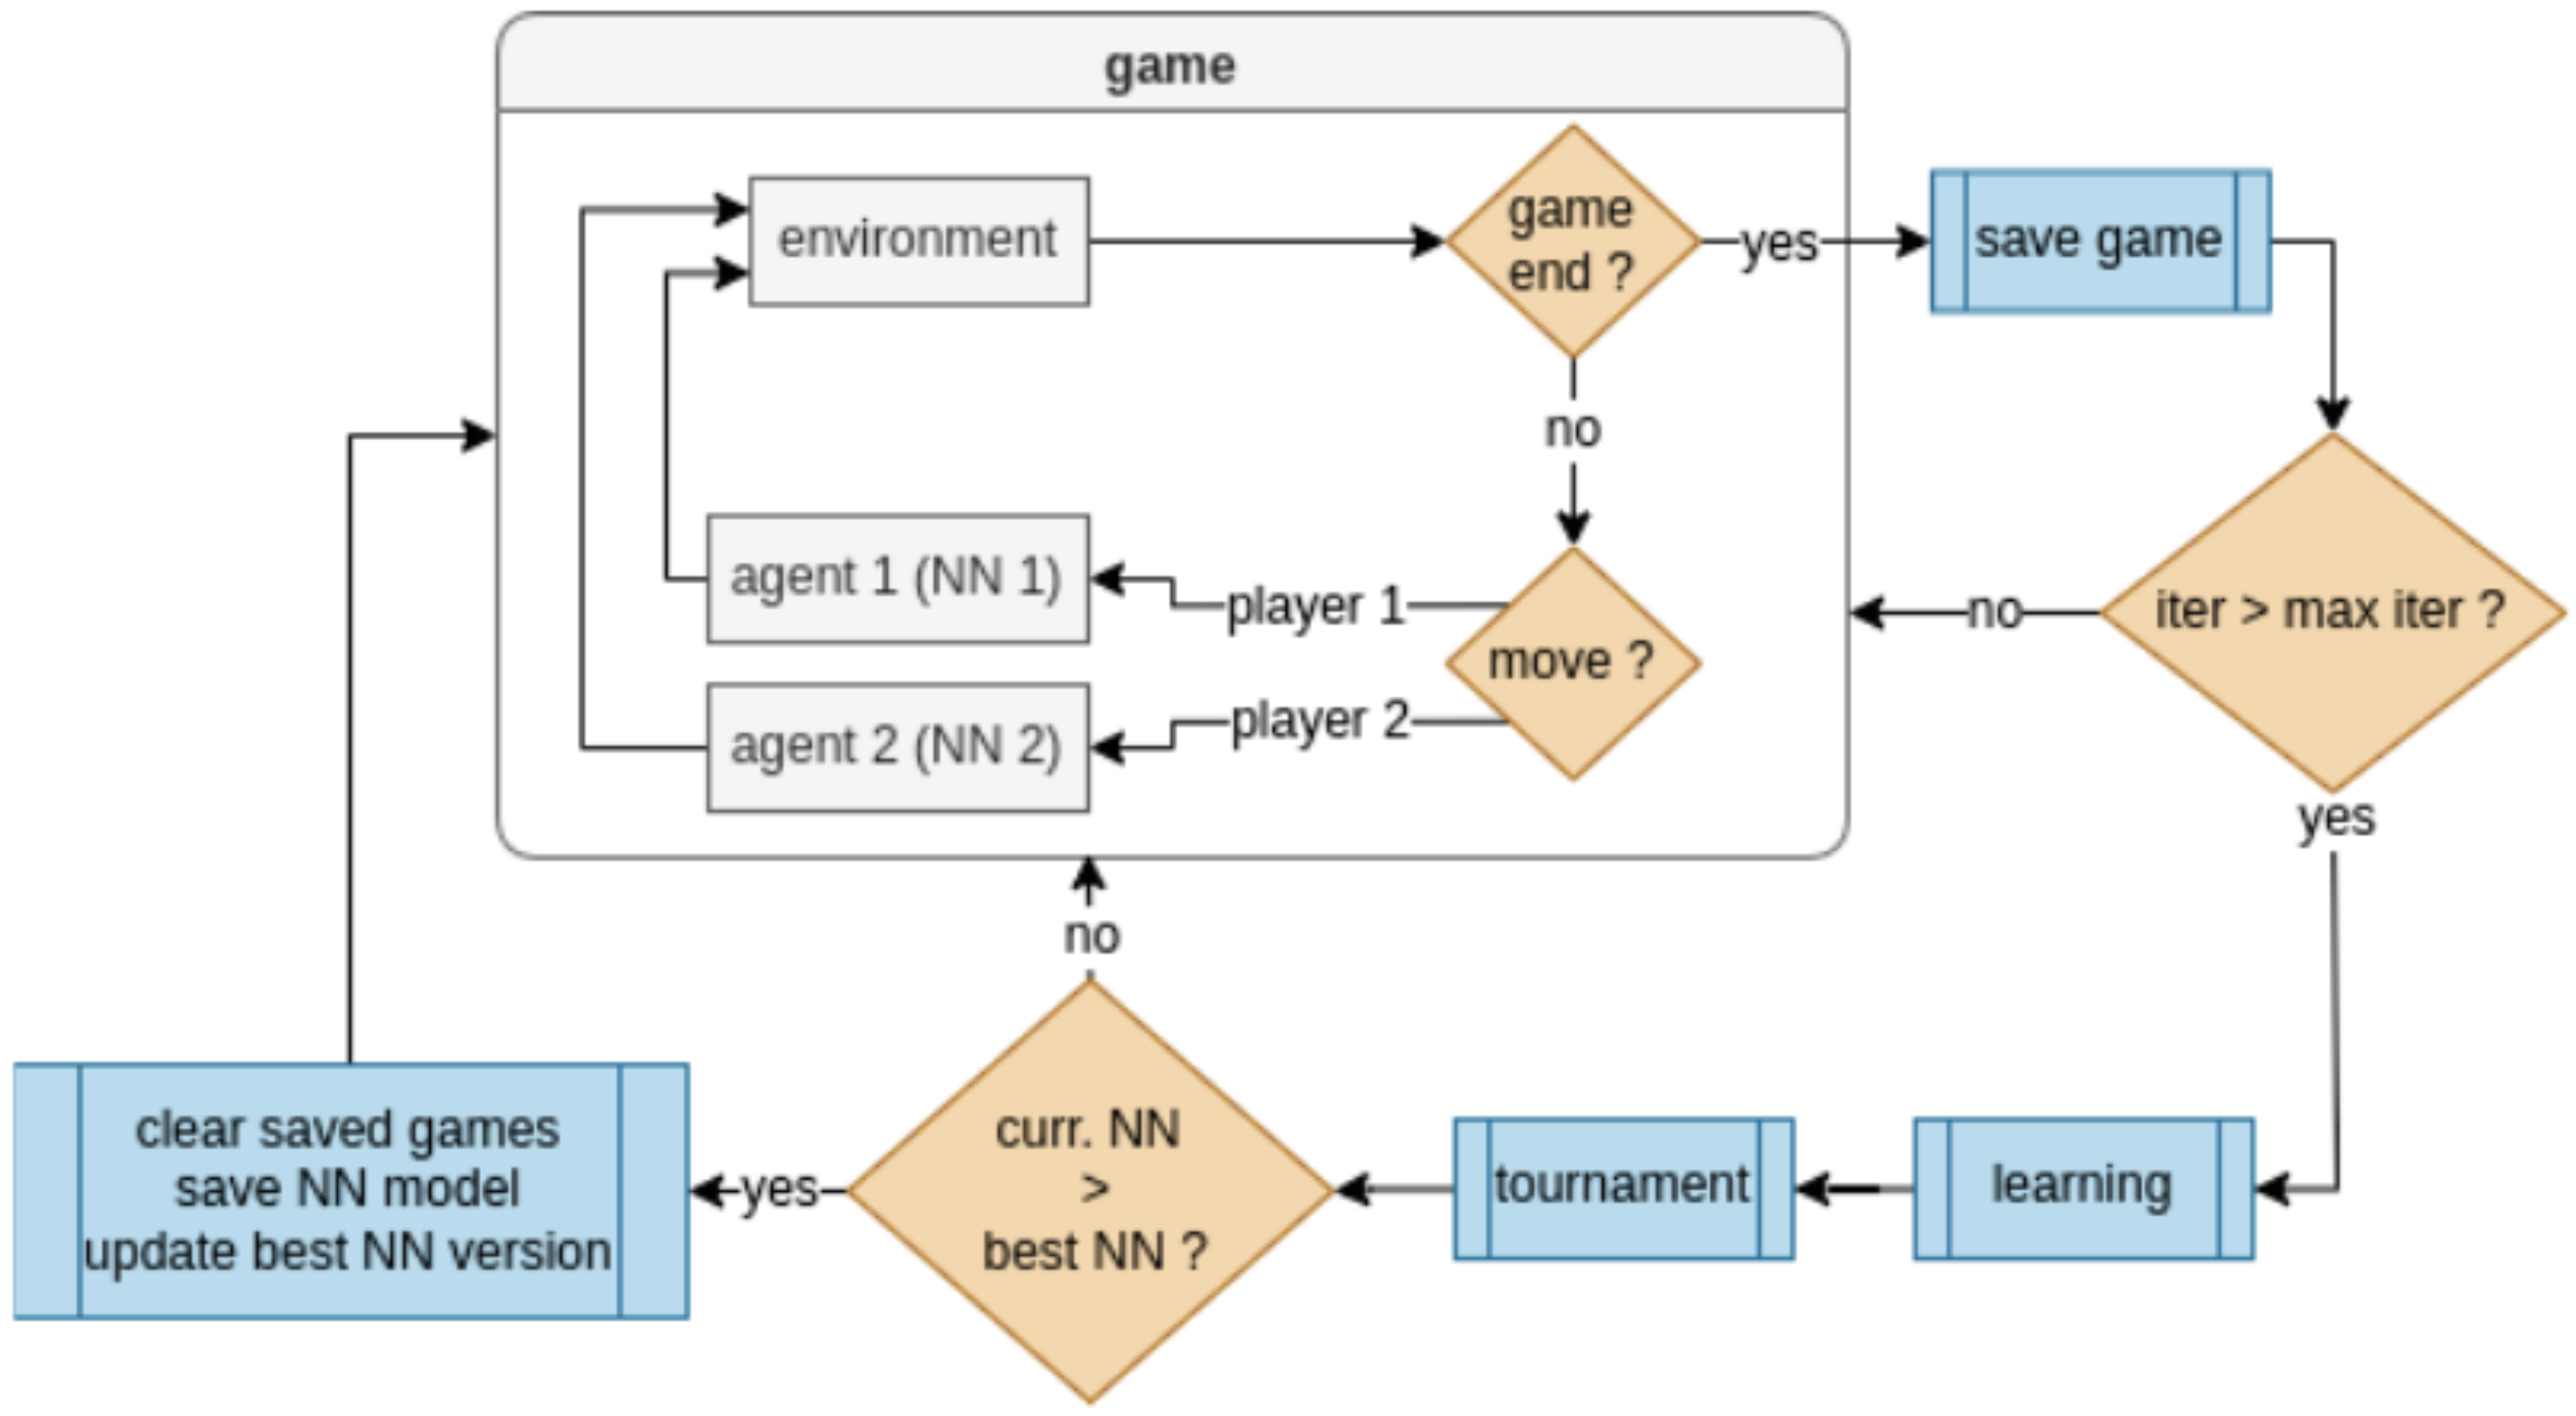
\includegraphics[width=0.7\linewidth]{images/self-play.png}
    \caption{General Flow Chart in \cite{Popic_Boskovic_Brest_2021}}
    \label{fig:self-play}
\end{figure}

After the data creation phase, the learning phase is initialized. During this phase, the generated data is used to train the current neural network with reinforcement learning combined with input batches.

After the learning phase, a tournament is started between the agent using the newly trained neural network and the one using the currently best neural network. During the tournament phase, \verb!EVAL_EPISODES! games are played. Each agent is scored according to the chess scoring where 3 points is given for a win, 1 point for a draw and 0 points for a loss. The newly trained neural network is deemed the current best if the agent using the newly trained neural network has obtained more points than the agent using the currently best neural network by a ratio defined by the \verb!SCORING_THRESHOLD! parameter after the completion of the tournament phase and the whole process is repeated again.

\cite{Popic_Boskovic_Brest_2021} ran the algorithm as described with parameters seen in Table \ref{tab:algo-params}. Instead of discarding the older neural network model when a better one was found, \cite{Popic_Boskovic_Brest_2021} saved that version for later use. After approximately 2 weeks of runtime, \cite{Popic_Boskovic_Brest_2021} were able to obtain 9 different versions of the neural network model, each being better than the previous one. \cite{Popic_Boskovic_Brest_2021} ran fifty games between an agent using the ninth version of the neural network model marked as the best and agents using every other versions of the neural network. Every game was scored according to the chess scoring. Number of wins (W), draws (D), and losses(L) of the ninth version of the neural network versus other versions as well as the final score (S) can be seen in Table \ref{tab:v9_summary}.

\begin{table}[htb]
    \centering
    \begin{tabular}{c|cccccccccc}
        & v0 & v1 & v2 & v3 & v4 & v5 & v6 & v7 & v8 & v9 \\ \hline
        W & 32 & 27 & 26 & 33 & 29 & 26 & 18 & 11 & 14 & 17 \\
        D & 13 & 18 & 19 & 10 & 17 & 13 & 16 & 20 & 14 & 16 \\
        L & 5 & 5 & 5 & 7 & 4 & 11 & 16 & 19 & 22 & 17 \\ \hline
        S & 109 & 99 & 97 & 109 & 104 & 91 & 70 & 53 & 56 & 67
    \end{tabular}
    \caption{Games of the Agent using the Ninth Version of the Neural Network Against All Other Versions of the Neural Network in \cite{Popic_Boskovic_Brest_2021}}
    \label{tab:v9_summary}
\end{table}

The final scores against lower and worse versions of the neural network are generally higher than those against higher and better versions. The number of wins generally decreases and the number of losses generally increases. The ninth version of the neural network obtained the same number of wins and losses when playing against itself, as shown in the ninth column of Table \ref{tab:v9_summary}, which is on par with the idea that two equivalent players will have the same chances of winning and losing.

The paper by \cite{Popic_Boskovic_Brest_2021} managed to demonstrate the ability of an AlphaZero-based approach to learning the game of Checkers when given only the game rules. The approach is only given a set of game rules. The data needed to train newer models of neural network are generated by self-play. Nine different versions of the neural network were obtained after two weeks of runtime, each better than the previous one. Some discrepancies are seen with regards to the score achieved by the first few versions, which is most likely due to noise and could be addressed by optimizing the \verb|EPISODES|, \verb|EVAL_EPISODES|, and \verb|SCORING_THRESHOLD| parameters according to \cite{Popic_Boskovic_Brest_2021}.


\section{The Game of Damath}

Damath comes from the Filipino checkers called ``dama'' and mathematics. According to \cite{MathleteSociety2024}, Damath was created by Jesus Huenda, a teacher in the province of Sorsogon, Philippines who was inspired by his student named Emilio Hina Jr. for his submission of an investigatory project called ``Dama de Numero'' in 1975. Huenda developed and refined the game, first introducing it to his students. The popularity of the game grew rapidly, leading to the first Damath tournament being held in Sorsogon in 1980.  The innovative approach of Huenda to teaching mathematics earned him a gold medallion from the late President Ferdinand Marcos in 1981. The popularity of Damath reached its peak in the 1990s, with the game being featured at numerous mathematics education conventions around the world, including conferences in Australia, Thailand, Malaysia, and Korea. In 2011, Damath was introduced to the United States by Reynaldo L. Duran, an international Filipino educator, at the National Council of Teachers of Mathematics (NCTM) conference in New Mexico.

Damath is very similar to the game of Checkers, except that the checkerboard has the basic mathematical operations (addition, subtraction, multiplication and division) on each playable tiles which dictates the operation that will be used when a piece of a player captures the piece of an opponent. It has numbers labeled 0-7 on its sides to determine the coordinates of the piece. Each piece of the player has corresponding values depending on what type of damath is being played. Both board and damath pieces are mostly made of thick cardboard or illustration board.

\begin{figure}[htb]
     \centering
     \includegraphics[width=0.5\linewidth]{images/initial_state.png}
     \caption{Initial State of Damath}
     \label{fig:initial_state}
\end{figure}
 
If there is an opponent's figure in the path of the move and the square behind that figure is vacant, the player must capture the opponent's figure by jumping over it and removing it from the playing board. The capturing figure must perform a calculation based on the mathematical operator where the capturing figure lands. If multiple such successive captures exist, the player must perform them all in one move. The result of the calculation is added to the score of the player who captured the piece.

If the player reaches opponent’s side of the board, the player's figure turns into a dama and hence has the ability to move diagonally forward and backward. Game is won if the opponent has no figures left on the board or is out of possible legal moves. The game ends in a draw if no pieces have been captured in the last 40 moves.
 

\section{Existing AI Models for Damath}

Although AI in Damath is less explored than in other board games, a few existing models attempt to simulate intelligent play within the rules of the game. These models are often based on rule-based algorithms or basic decision trees that follow predefined strategies. However, they have limitations, particularly in their inability to adapt dynamically to player strategies or to demonstrate the flexibility required for challenging higher-level human players.

Most existing Damath AIs rely on rule-based algorithms, which hardcode responses to specific game states. These models are effective at teaching basic strategies but lack the ability to innovate or surprise players, resulting in a predictable gameplay experience. This limitation reduces the value of AI value as a learning tool for advanced players seeking a more challenging opponent.

Traditional Damath AI models lack the complexity and adaptability required for advanced strategic thinking. These models do not self-improve or adapt over time, which means players cannot experience the progression and increasing difficulty found in the reinforcement learning approach of AlphaZero. The introduction of AlphaZero to Damath offers a potential solution to this problem by creating an AI that evolves with experience, providing a continuous challenge to players as they improve.